\chapter{Resultados}
\label{results}

En este capítulo se presentan los \textbf{resultados obtenidos} tras el desarrollo e implementación del proyecto. Se detallan los \textbf{principales logros alcanzados, el funcionamiento de las distintas funcionalidades desarrolladas y el comportamiento general de la aplicación} en diferentes escenarios de uso.
\\\\
Además, se incluyen capturas de pantalla, descripciones funcionales y observaciones relevantes que permiten evaluar el grado de cumplimiento de los objetivos planteados en capítulos anteriores, así como identificar posibles mejoras o líneas de trabajo futuras.

\section{Funcionalidades conseguidas}

De las funcionalidades definidas en un principio, se han conseguido los siguientes objetivos:

\begin{itemize}
    \item Se ha comprendido el funcionamiento interno de la consola.
    \item Se ha diseñado una arquitectura modular y escalable, pensada para futuras ampliaciones.
    \item Se ha implementado una interfaz gráfica funcional, adaptable y coherente.
    \item Se ha documentado de forma detallada todo el proceso de desarrollo en esta memoria.
\end{itemize}

En general, el producto obtenido cumple con el objetivo principal: el usuario es capaz de ejecutar y jugar ROMs cuyos MBCs sean de los tipos \textbf{NoMBC} o \textbf{MBC1}. Esta característica permite la ejecución de títulos conocidos como \textit{Tetris DX}, \textit{Wario Land} o \textit{Super Mario Land 2}.
\\\\
La interfaz gráfica es simple, funcional y se adapta correctamente a diferentes resoluciones de pantalla. Además, el simple hecho de poder jugar a \textit{Tetris} ya representa, en sí mismo, un objetivo cumplido.

\begin{figure}[H]
    \centering
    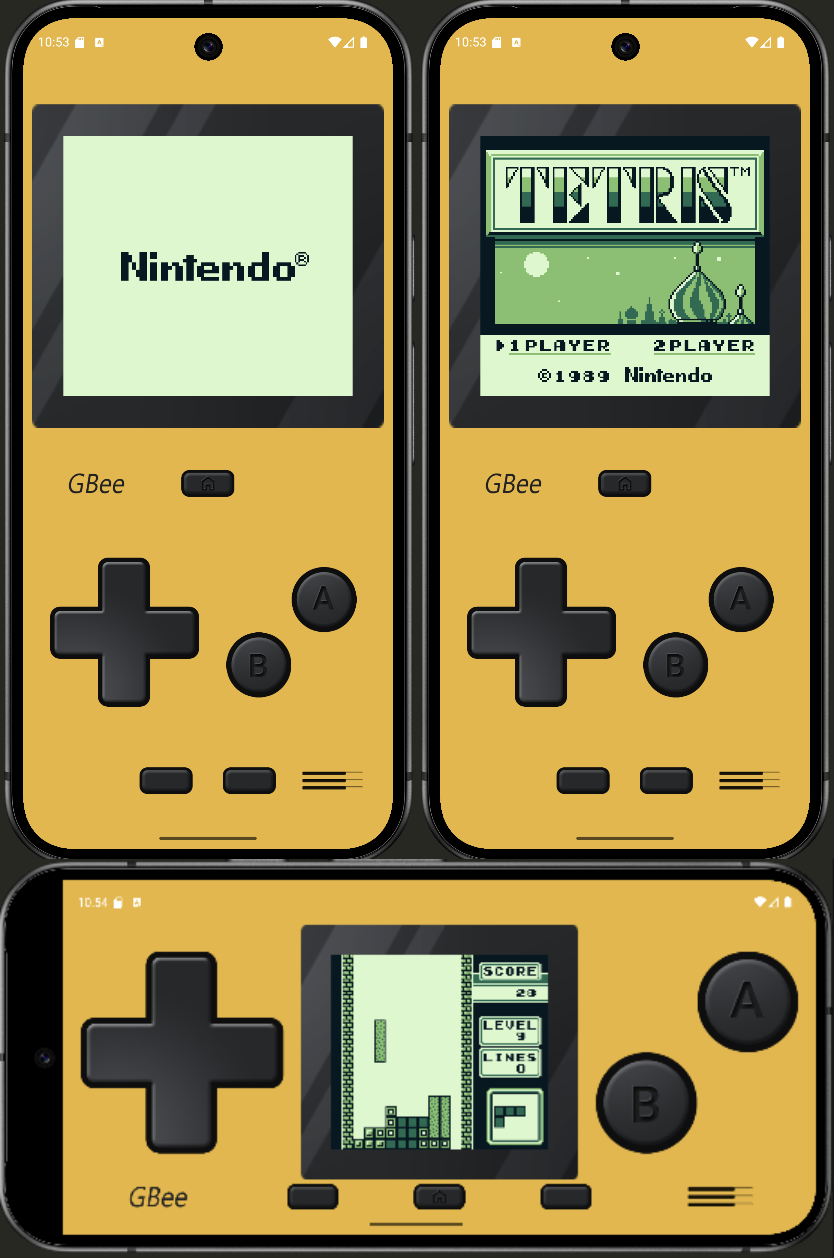
\includegraphics[width=0.6\textwidth]{include/images/results_emu.png}
    \caption{Resultado de la Pantalla de Juego de la Aplicación.}\label{figure:resultemu}
\end{figure}

\section{Posibles Mejoras}

\textbf{La aplicación}, en su estado actual, \textbf{cumple su propósito} tanto como emulador funcional como herramienta de aprendizaje sobre el hardware de la Game Boy. Sin embargo, es importante identificar qué elementos no se han llegado a implementar o qué aspectos podrían mejorarse en futuras versiones:

\begin{itemize}
    \item \textbf{Módulo de audio}. El sonido es un componente esencial en cualquier videojuego. Aunque se tuvo en cuenta desde el inicio, su implementación fue descartada en las últimas fases para centrarse en consolidar el funcionamiento general del emulador.
    
    \item \textbf{Compatibilidad con más tipos de MBC}. Actualmente solo se soportan los tipos \textbf{NoMBC} y \textbf{MBC1}. Para ampliar el catálogo de juegos compatibles, será necesario implementar soporte para otros tipos como MBC2, MBC3, MBC5, entre otros.
    
    \item \textbf{Publicación en la Play Store}. Aunque se definió como una funcionalidad deseada, debido a la falta de algunas características clave y a la intención de seguir puliendo el proyecto, se decidió posponer la publicación.
    
    \item \textbf{Sistema de configuración avanzada}. A día de hoy, el usuario puede modificar aspectos básicos como el título del juego, la portada o algunos elementos de la interfaz. Sin embargo, se echan en falta opciones como ajustes gráficos o de audio.
    
    \item \textbf{Guardado y carga de partidas}. No es posible guardar ni cargar el estado de una partida. Cada sesión comienza desde el inicio, lo que puede no suponer un problema en juegos sin sistema de guardado, pero limita la experiencia en títulos más largos.
    
    \item \textbf{Errores gráficos}. Debido a una implementación personalizada del módulo gráfico, se producen desajustes visuales en ciertas circunstancias, como al desplazar la pantalla en horizontal. En particular, los \textit{tiles} del componente \textit{Window} pueden presentar un desfase constante.
    \item \textbf{Botón de \textit{Home} en la pantalla de juego}. El botón está contemplado en el código. Sin embargo, actualmente no funciona, por lo que para retroceder de la actividad el usuario debe hacer uso del botón de retroceso propio de Android. Este botón debe dar también las opciones de guardar o cargar la partida.
\end{itemize}

\section{Estimaciones}\label{estimaciones}

En un principio, se estimó que el desarrollo estaría finalizado en torno al 8 de diciembre, con la memoria completada para el 12 de enero. Aunque estas previsiones eran inicialmente realistas, diversos problemas personales y la dificultad de compaginar los estudios con el trabajo provocaron un retraso de aproximadamente tres meses respecto al calendario previsto.
\\\\
Además, durante el mes de enero, el proyecto sufrió un parón significativo debido a las dificultades para comprender en profundidad el funcionamiento de la PPU y su gestión del procesamiento gráfico. Sin duda, este ha sido el apartado técnico que más esfuerzo ha requerido a lo largo del desarrollo.

\cleardoublepage
\chapter{Conclusiones}
\label{conclusiones}

En primer lugar, puedo afirmar que estoy \textbf{satisfecho con los resultados obtenidos}. Aunque soy consciente de que aún queda trabajo por hacer y funcionalidades por implementar, considero que el resultado actual representa \textbf{un buen producto}, fruto de muchas horas de \textbf{dedicación y esfuerzo}.
\\\\
Tal y como se menciona en el apartado de \hyperref[estimaciones]{\textbf{estimaciones}}, \textbf{el mayor reto técnico ha sido, sin duda, la implementación de la PPU}. A pesar de leer abundante documentación disponible en internet, me resultaba difícil comprender cómo llevar a la práctica ciertos conceptos clave. Afortunadamente, encontré una serie de vídeos que ofrecían una implementación alternativa, \textbf{más accesible tanto en su explicación como en su desarrollo}, lo que me permitió superar ese bloqueo.
\\\\
\textbf{Esta experiencia me ha hecho valorar aún más el trabajo de aquellos desarrolladores} que, sin apenas referencias o documentación previa, logran emular consolas desde cero.
\\\\
En mi caso, al haber cursado el máster en dos años, pude comenzar el proyecto durante los tres meses de verano, antes de que comenzaran de nuevo las clases. Por ello, las estimaciones iniciales contemplaban finalizar el desarrollo en enero. Sin embargo, a medida que avanzaba el curso, las prácticas del resto de asignaturas comenzaron a acumularse una tras otra, lo que provocó que el proyecto \textbf{sufriera parones semanales de forma constante}. Esta situación es algo que \textbf{debería haber previsto desde el principio}, y sin duda es \textbf{una lección importante que me llevo sobre planificación y gestión del tiempo}.
\\\\
Este proyecto también me ha hecho reflexionar sobre la \textbf{importancia de cuidar mi salud}. Aunque aún soy joven, he aprendido que no se puede dar por sentado algo tan fundamental como el \textbf{bienestar físico y mental}. Compaginar el trabajo con la universidad ha implicado pasar la mayoría de los días sentado en la misma silla, desde las ocho de la mañana hasta las nueve de la noche. Este ritmo de vida ha terminado afectando a mi salud, y me ha hecho comprender que, en el futuro, \textbf{debo priorizarme más a mí mismo}. \textbf{Ningún proyecto o trabajo vale más que la salud}.
\\\\
A pesar de todas las dificultades, \textbf{la experiencia a lo largo del curso ha sido muy gratificante}. Considero que he logrado desarrollarme tanto a nivel profesional como personal, y que termino esta etapa con una \textbf{mayor madurez como ingeniero}. Todo lo aprendido me ha permitido \textbf{ampliar significativamente el abanico de posibilidades laborales} en las que puedo desenvolverme, y que también pienso aplicar en \textbf{futuros proyectos personales}.

